% !TEX program = pdflatex
% !TEX options = -synctex=1 -interaction=nonstopmode -file-line-error "%DOC%"
% Computational Physics Assignment 1
\documentclass[UTF8,10pt,a4paper]{article}
\usepackage{ctex}
\newcommand{\CourseName}{Computational Physics}
\newcommand{\CourseCode}{PHYS1504}
\newcommand{\Semester}{Spring, 2020}
\newcommand{\ProjectCode}{Assignment 1}
\newcommand{\ProjectName}{One-dimensional Schrödinger equation}
\newcommand{\DueTimeType}{Due Time}
\newcommand{\DueTime}{23:59, March 15, 2020 (Sunday)}
\newcommand{\StudentName}{陈稼霖}
\newcommand{\StudentID}{45875852}
\usepackage[vmargin=1in,hmargin=.5in]{geometry}
\usepackage{fancyhdr}
\usepackage{lastpage}
\usepackage{calc}
\pagestyle{fancy}
\fancyhf{}
\fancyhead[L]{\CourseName}
\fancyhead[C]{\ProjectCode}
\fancyhead[R]{\StudentName}
\fancyfoot[R]{\thepage\ / \pageref{LastPage}}
\setlength\headheight{12pt}
\fancypagestyle{FirstPageStyle}{
    \fancyhf{}
    \fancyhead[L]{\CourseName\\
        \CourseCode\\
        \Semester}
    \fancyhead[C]{{\large\bfseries\ProjectCode}\\
        {\large\bfseries\ProjectName}\\
        \DueTimeType\ : \DueTime}
    \fancyhead[R]{Name : \makebox[\widthof{\StudentID}][s]{\StudentName}\\
        Student ID\@ : \StudentID\\
        Score : \underline{\makebox[\widthof{\StudentID}]{}}}
    \fancyfoot[R]{\thepage\ / \pageref{LastPage}}
    \setlength\headheight{36pt}
}
\usepackage{amsmath,amssymb,amsthm,bm}
\allowdisplaybreaks[4]
\newtheoremstyle{Problem}
{}
{}
{}
{}
{\bfseries}
{.}
{ }
{\thmname{#1}\thmnumber{ #2}\thmnote{ (#3)} Score: \underline{\qquad\qquad}}
\theoremstyle{Problem}
\newtheorem{prob}{Problem}
\newtheoremstyle{Solution}
{}
{}
{}
{}
{\bfseries}
{:}
{ }
{\thmname{#1}}
\makeatletter
\def\@endtheorem{\qed\endtrivlist\@endpefalse}
\makeatother
\theoremstyle{Solution}
\newtheorem*{sol}{Solution}
\providecommand{\abs}[1]{\left\lvert#1\right\rvert}
\usepackage{listings}
\lstset{language=[95]Fortran,
numbers=left,
frame=single,
breaklines=true}
\usepackage{booktabs}
\usepackage{array}
\usepackage{multirow}
\usepackage{ulem}
\usepackage{graphicx}
\begin{document}
\thispagestyle{FirstPageStyle}
\begin{prob}
    Suppose there is a single particle of mass $m$ confined to $0<x<L$ with potential $V=0$ bounded by infinite high potential barrier, \textit{i.e.}
    \begin{align*}
         & V(x)=0\quad\text{where }0<x<L,
         & V(x)=\infty\quad\text{where }x\geq L; x\leq 0
    \end{align*}
    \begin{enumerate}
        \item[(a)] Program Numerov's method for this type of potential. (hint: stat with the 1D harmonic oscillator code and update the potential function.) (\textbf{2 points})
        \item[(b)] Determine the first three lowest energies and the corresponding wave function. (\textbf{1 points})
        \item[(c)] Compare your results to the exact solution analytically obtained in quantum mechanics. (\textbf{1 points})
              \begin{gather}
                  E_n=\frac{(n\pi\hbar)^2}{2mL^2}\\
                  \begin{align}
                      \nonumber\Psi_n(x)= & \sqrt{\frac{2}{L}}\sin(n\pi x/L) &  & 0<x<L            \\
                      =                   & 0                                &  & x\leq 0, x\geq L
                  \end{align}
              \end{gather}
    \end{enumerate}
\end{prob}
\begin{sol}
    \begin{enumerate}
        \item[(a)] 由于势能$V$在$[0,L]$范围以外为无穷大,因此波函数在$[0,L]$范围以外均为零,而仅在$[0,L]$范围内不为零,且由连续性条件在两个端点$x=0$和$x=L$处为零. 为用Numerov方法求解在这一势场下粒子的薛定谔方程,只需在原来求解谐振子方程的代码的基础上,将波函数自变量\verb|x|的取值范围由\verb|[-Xmax,Xmax]|改为\verb|[0,L]|,并将\verb|Vpot|删去(因为存储势能函数的\verb|Vpot|在要计算的\verb|[0,L]|范围内为零). 简单起见,设$\hbar$,$L$,$m$在国际单位制下的数值均为$1$. 计算步骤(步骤后括号内数字为对应代码行号):
              \begin{itemize}
                  \item 给定所要计算的区域范围$[-Xmax,Xmax]$,离散化的数量$Nx$,以及能量$E$的尝试值(19--26);
                  \item 给定开始两点的波函数值作为迭代初始值(44--45);
                  \item 计算各处的函数值$g(x_i)$和$s(x_i)$,从而用numerov方法迭代得到各点的波函数值(47-55);
                  \item 归一化计算得到的波函数(58-59);
                  \item 检查是否$y_N=0$,若是,则将结果写入文件并退出程序,否则重新选定能量$E$的值,再次计算(65-110).
              \end{itemize}
              Fortran代码:
              \begin{lstlisting}
program main
    ! solve the Schrodinger equation of a particle in 1-dimension infinite square potential well with Numerov's method

    implicit none
    integer, parameter :: dp = selected_real_kind(8)
    real(dp), parameter :: eps = 1.d-5, dE = 1.d-2

    ! local vars
    real(dp) :: L = 1.d0
    integer :: Nx, i
    real(dp) :: E    ! trial energy
    real(dp) :: dx, ySquareSum
    real(dp), allocatable :: x(:), y(:), g(:), f(:)
    logical :: yNSignChange = .false., yNSign
    integer :: looptime = 1
    real(dp) :: Eprev1, Eprev2, yprev1, yprev2

    ! executable
    Nx = -1
    do while ((Nx <= 0) .or. (mod(Nx, 2) /= 0))
        write(*,*) 'Please specify the # of slices between [0,L] (must be a even integer), Nx ='
        read(*,*) Nx
    end do

    write(*,*) 'Please give a trial energy E0, the first allowed state with E>E0 will be calculated! E0 ='
    read(*,*) E

    write(*, '(a10,a20,a20)') 'Iteration', 'Energy', 'Boundary value'

    ! memory dynamical allocation
    allocate(x(0:Nx))
    allocate(y(0:Nx))
    allocate(g(0:Nx))
    allocate(f(0:Nx))

    dx = L / dble(Nx)
    do i = 0, Nx
        x(i) = dx * i
        ! Vpot(i) = .5d0 * x(i)**2
    end do

    do while (.true.)
        ! set boundary condition: y(0) and y(1)
        y(0) = 0.d0
        y(1) = 1.d-4

        do i = 0, Nx
            g(i) = 2.d0 * E
            f(i) = 1.d0 + g(i) / 12.d0 * dx**2
        end do

        ! Numerov's method
        do i = 1, Nx - 1
            y(i + 1) = ((12.d0 - 10.d0 * f(i)) * y(i) - f(i - 1) * y(i - 1)) / f(i + 1)
        end do

        ! renormalize y(x)
        call Simpson(Nx + 1, y(:), dx, ySquareSum)
        y = y / sqrt(ySquareSum)

        ! output to screen
        write(*,'(i10,2f20.8)') looptime, E, y(Nx)

        ! change E
        if (abs(y(Nx)) < eps) then    ! if precision requirement is satisfied
            ! output to file
            open(1, file = '1-wavefunction.txt', status = 'unknown')
            do i = 0, Nx
                write(1, '(2f20.8)') x(i), y(i)
            end do
            close(1)
            open(2, file = '1-energy.txt', status = 'unknown')
            write(2, '(f20.8)') E
            close(2)
            exit
        else
            if (.not. yNSignChange) then    ! if the sign of yN has not changed
                E = E + dE
                if (looptime == 1) then    ! if this is the first loop
                    yNSign = (y(Nx) >= 0)
                    yprev1 = y(Nx)
                else
                    if ((y(Nx) >=0) .neqv. (yNSign)) then    ! if the sign of yN changed this time
                        yNSignChange = .true.
                        E = E - dE
                        Eprev1 = E
                        Eprev2 = E - dE
                        E = E - dE / 2.d0
                    end if
                    yprev2 = yprev1
                    yprev1 = y(Nx)
                end if
            else    ! once the sign of yN has changed
                if (abs(yprev1) <= abs(yprev2)) then
                    Eprev2 = E
                    ! Eprev1 = Eprev1
                    E = (Eprev1 + Eprev2) / 2.d0
                    yprev2 = y(Nx)
                    ! yprev1 = yprev1
                else
                    ! Eprev2 = Eprev2
                    Eprev1 = E
                    E = (Eprev1 + Eprev2) / 2.d0
                    ! yprev2 = yprev2
                    yprev1 = y(Nx)
                end if
            end if
        end if

        looptime = looptime + 1
    end do
end program main

subroutine Simpson(N, y, dx, ySquareSum)
    ! calculate the integral of the square of the wavefunction from -Xmax to Xmax with compound simpson formula

    implicit none
    integer :: N
    real(8), intent(in) :: y(N), dx
    real(8), intent(out) :: ySquareSum

    ! local vars
    integer :: i
    real(8) :: Work(N)

    if (mod(N,2) == 0) then
    ! Simpson does not work for integral of array with even number of elements
        write(*, *) 'Array with even elements, Simpson does not know how to work!'
    end if

    do i = 1,N
        Work(i) = y(i)**2
    end do

    ySquareSum = Work(1) + Work(N)
    do i = 2, N - 1, 2
        ySquareSum = ySquareSum + 4.d0 * Work(i)
    end do
    do i = 3, N - 2, 2
        ySquareSum = ySquareSum + 2.d0 * Work(i)
    end do
    ySquareSum = ySquareSum * dx / 3.d0

end subroutine Simpson
        \end{lstlisting}
              \newpage
        \item[(b)] 用以上代码计算最低的三个能级能量和对应的波函数,结果如表\ref{1-2}所示.
              \begin{table}[h]
                  \centering
                  \caption{计算结果:一维无限深方势阱最低的三个能级能量和对应的波函数.}
                  \label{1-2}
                  \begin{tabular}{ccm{.4\textwidth}}
                      \hline
                      能级序号 & \begin{tabular}[c]{@{}c@{}}能量\\ (国际单位制)\end{tabular} & \begin{tabular}[c]{@{}c@{}}$[0,L]$范围内波函数图像\\ ($[0,L]$范围外波函数均为零)\end{tabular}                       \\ \hline
                      1        & $4.93480469$              & 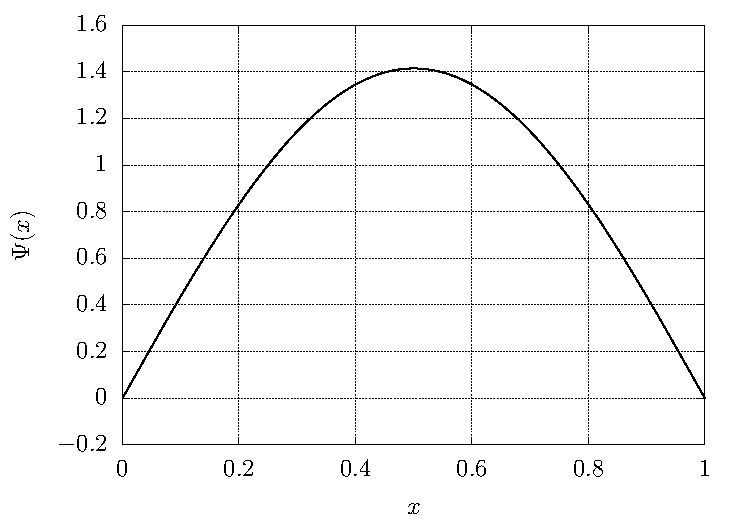
\includegraphics[width=.4\textwidth]{1-2-1.pdf} \\
                      2        & $19.73921875$             & 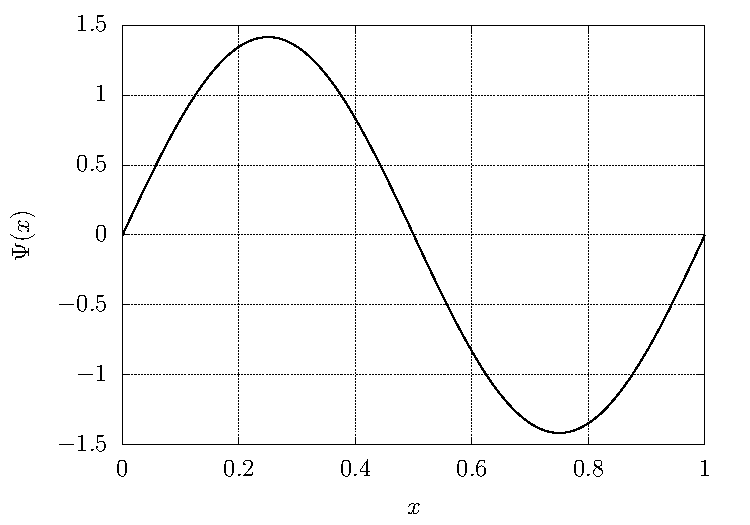
\includegraphics[width=.4\textwidth]{1-2-2.pdf} \\
                      3        & $44.41328125$             & 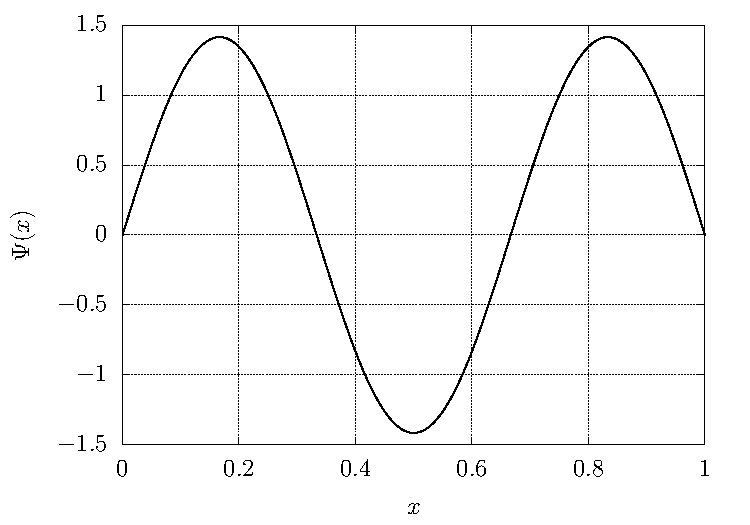
\includegraphics[width=.4\textwidth]{1-2-3.pdf} \\ \hline
                  \end{tabular}
              \end{table}
              \newpage
        \item[(c)] 我们通过一下步骤比较Numerov方法计算结果与其精确值:
              \begin{itemize}
                  \item 计算各能级能量的精确值;
                  \item 计算各能级能量计算值相对于其精确值的误差;
                  \item 计算各点的波函数精确值(计算所用节点与(a)中所用节点相同),将波函数计算值和精确解的绘制在同一张图中比较;
                  \item 计算波函数计算值相对于其精确值的误差,这里两条曲线之间的误差定义为各点计算值与当地精确值的欧几里得距离平均值.
              \end{itemize}
              比较结果如表\ref{1-3}.
              \begin{table}[h]
                  \caption{比较:计算结果和精确值}
                  \label{1-3}
                  \begin{tabular}{cccccm{.33\textwidth}c}
                      \hline
                      \multirow{2}{*}{\begin{tabular}[c]{@{}c@{}}能级\\ 序号\\ $n$\end{tabular}} & \multicolumn{3}{c}{\begin{tabular}[c]{@{}c@{}}能量$E_n$\\ (国际单位制)\end{tabular}} &                           & \multicolumn{2}{c}{波函数$\Psi_n(x)$}                                                                                    \\ \cline{2-4} \cline{6-7}
                                                                 & 计算值                                        & \begin{tabular}[c]{@{}c@{}}精确值\\ $\frac{(n\pi\hbar)^2}{2mL^2}$\end{tabular} & 相对误差                              &  & \begin{tabular}[c]{@{}c@{}}$[0,L]$范围内函数图像\\ (“$+$”代表计算所得函数值,\\ 实线代表精确波函数曲线,\\ $[0,L]$范围外波函数均为零)\end{tabular}                       & 误差                       \\ \hline
                      $1$                                        & $4.93480469$                                  & $4.93480220$              & $0.00005\%$                           &  & 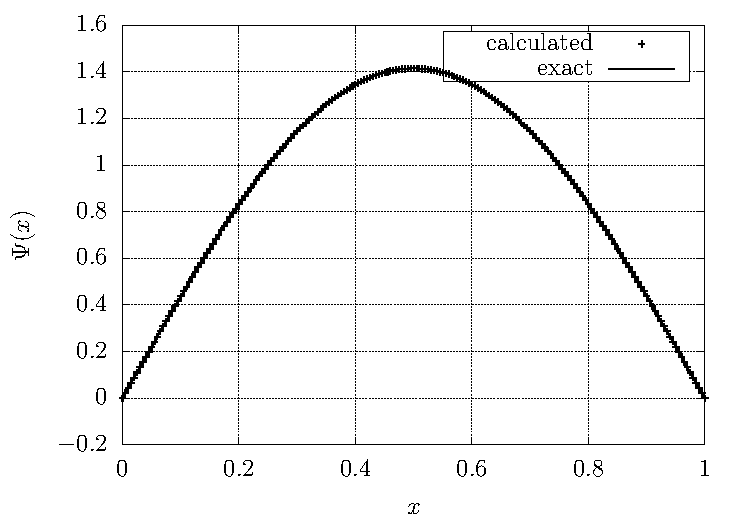
\includegraphics[width=.33\textwidth]{1-3-1.pdf} & $3.74129353\times 10^{-7}$ \\
                      $2$                                        & $19.73921875$                                 & $19.73920880$             & $0.00005\%$                           &  & 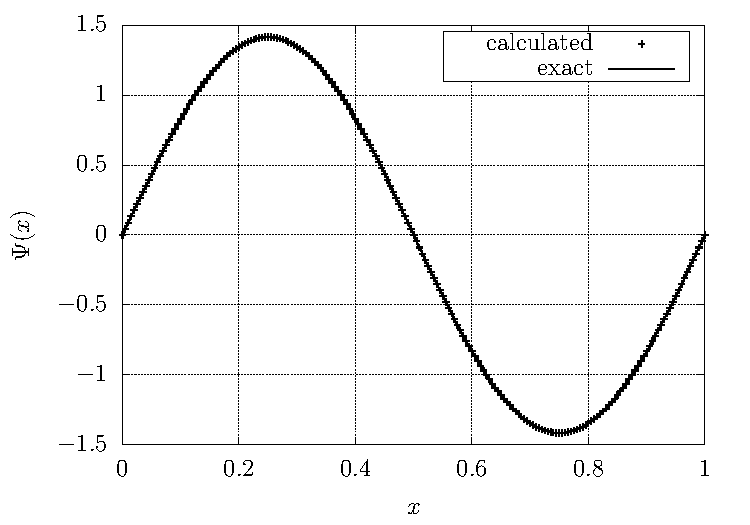
\includegraphics[width=.33\textwidth]{1-3-2.pdf} & $7.31393035\times 10^{-7}$ \\
                      $3$                                        & $44.41328125$                                 & $44.41321980$             & $0.00014\%$                           &  & 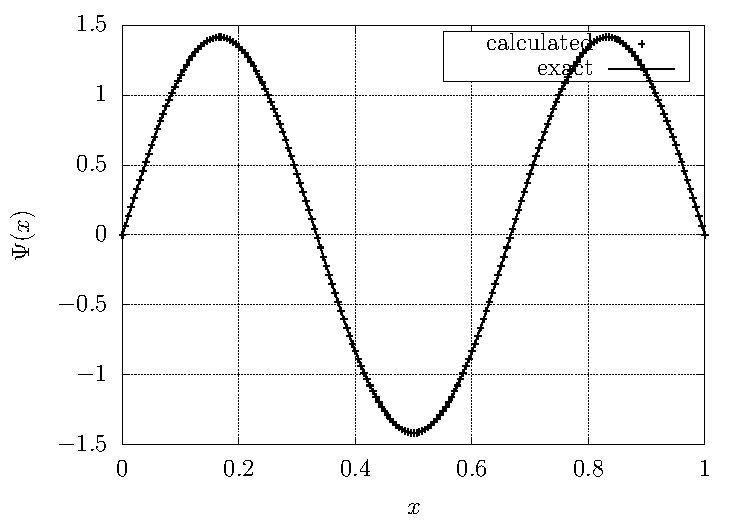
\includegraphics[width=.33\textwidth]{1-3-3.pdf} & $3.00985075\times 10^{-6}$ \\ \hline
                  \end{tabular}
              \end{table}
              \\无论从误差的数值还是波函数的图像上,均可见Numerov方法计算所得结果十分精确.
    \end{enumerate}
\end{sol}

\begin{prob}
    Prove the energy of the matrix Schrödinger equation on non-orthogonal basis states satisfies the variation principle as well. (\textbf{3 points})
\end{prob}
\begin{proof}
    在一组非正交的基上,系统的波函数可展开为
    \begin{equation}
        \Psi(x)=\sum_kc_k\Psi_k(x).
    \end{equation}
    我们定义两个基矢的内积为
    \begin{equation}
        \int_{-\infty}^{+\infty}\Psi_k^*(x)\Psi_{k'}(x)\,dx=W_{kk'}.
    \end{equation}
    系统的能量可表为
    \begin{equation}
        \label{2-E}
        E=\frac{\langle\Psi(x)\rvert H\lvert\Psi(x)\rangle}{\langle\Psi(x)\vert\Psi(x)\rangle}=\frac{\sum_{kk'}c_k^*c_{k'}H_{kk'}}{\sum_{kk'}c_k^*c_{k'}W_{kk'}}.
    \end{equation}
    假设波函数展开式中第$q$项的系数发生微小改变:$c_q\rightarrow c_q+\delta_q$,对应地,该系数的复共轭变为:$c_q^*\rightarrow c_q^*+\delta_q^*$. 系统能量变为
    \begin{align}
        \nonumber        & (\text{分子和分母分别展开并忽略高阶小量})                                                                                                                                                                                                                                    \\
        \nonumber E'=    & \frac{\sum_{kk'}c_k^*c_{k'}H_{kk'}+\sum_k(c_k^*\delta_qH_{kq}+\delta_q^*c_kH_{qk})}{\sum_{kk'}c_k^*c_{k'}W_{kk'}+\sum_k(c_k^*\delta_qW_{kq}+\delta_q^*c_kW_{qk})}                                                                                                            \\
        \nonumber        & (\text{分母关于$\delta_q$和$\delta_q^*$应用泰勒展开,仅保留一阶项})                                                                                                                                                                                                          \\
        \nonumber\approx & \frac{\sum_{kk'}c_k^*c_{k'}H_{kk'}+\sum_k(c_k^*\delta_qH_{kq}+\delta_q^*c_kH_{qk})}{\sum_{kk'}c_k^*c_{k'}W_{kk'}}\times\left[1-\frac{\sum_k(\delta_qc_k^*W_{kq}+\delta_q^*c_kW_{qk})}{\sum_{kk'}c_k^*c_{k'}W_{kk'}}\right]                                                   \\
        \nonumber=       & \left[\frac{\sum_{kk'}c_k^*c_{k'}H_{kk'}}{\sum_{kk'}c_k^*c_{k'}W_{kk'}}+\frac{\sum_k(c_k^*\delta_qH_{kq}+\delta_q^*c_kH_{qk})}{\sum_{kk'}c_k^*c_{k'}W_{kk'}}\right]\times\left[1-\frac{\sum_k(\delta_qc_k^*W_{kq}+\delta_q^*c_kW_{qk})}{\sum_{kk'}c_k^*c_{k'}W_{kk'}}\right] \\
        \nonumber        & (\text{代入式\ref{2-E}})                                                                                                                                                                                                                                                     \\
        \nonumber=       & \left[E+\frac{\sum_k(c_k^*\delta_qH_{kq}+\delta_q^*c_kH_{qk})}{\sum_{kk'}c_k^*c_{k'}W_{kk'}}\right]\times\left[1-\frac{\sum_k(\delta_qc_k^*W_{kq}+\delta_q^*c_kW_{qk})}{\sum_{kk'}c_k^*c_{k'}W_{kk'}}\right]                                                                 \\
        \nonumber        & (\text{再次展开,仅保留一阶项})                                                                                                                                                                                                                                              \\
        =                & E+\frac{\sum_k(c_k^*\delta_qH_{kq}+\delta_q^*c_kH_{qk})}{\sum_{kk'}c_k^*c_{k'}W_{kk'}}-E\frac{\sum_k(c_k^*\delta_qW_{kq}+\delta_q^*c_kW_{qk})}{\sum_{kk'}c_k^*c_{k'}W_{kk'}}.
    \end{align}
    因为系统能量是一个稳定值,故在发生$c_k\rightarrow c_k+\delta_k$的微小变化时,系统能量变化值应为零:
    \begin{gather}
        E'-E=\frac{\sum_k(c_k^*\delta_qH_{kq}+\delta_q^*c_kH_{qk})}{\sum_{kk'}c_k^*c_{k'}W_{kk'}}-E\frac{\sum_k(c_k^*\delta_qW_{kq}+\delta_q^*c_kW_{qk})}{\sum_{kk'}c_k^*c_{k'}W_{kk'}}=0,\\
        \Longrightarrow\sum_k\delta_q^*c_kH_{qk}-E\sum_{k}\delta_q^*c_kW_{qk}+\text{c.c.}=0,\\
        \Longrightarrow\sum_kc_kH_{qk}=E\sum_kc_kW_{q,k}.
    \end{gather}
    考虑到$q$取值的任意性,上式对$q=1,2,\cdots,N$都成立:
    \begin{equation}
        \sum_kc_kH_{qk}=E\sum_kc_kW_{q,k},\quad q=1,2,\cdots.
    \end{equation}
    上式可以化为矩阵形式:
    \begin{gather}
        \left(\begin{matrix}
                H_{11} & H_{12} & \cdots & H_{1N} \\
                H_{21} & H_{22} & \cdots & H_{2N} \\
                \vdots & \vdots & \ddots & \vdots \\
                H_{N1} & H_{N2} & \cdots & H_{NN}
            \end{matrix}\right)\left(\begin{matrix}
                c_1    \\
                c_2    \\
                \vdots \\
                c_N
            \end{matrix}\right)=E\left(\begin{matrix}
                W_{11} & W_{12} & \cdots & W_{1N} \\
                W_{21} & W_{22} & \cdots & W_{2N} \\
                \vdots & \vdots & \ddots & \vdots \\
                W_{N1} & W_{N2} & \cdots & W_{NN}
            \end{matrix}\right)\left(\begin{matrix}
                c_1    \\
                c_2    \\
                \vdots \\
                c_N
            \end{matrix}\right),\\
        \Longrightarrow H\bm{c}=EW\bm{c}.
    \end{gather}
    因此由非正交基上的薛定谔矩阵式计算出的能量满足变分原理.
\end{proof}

\begin{prob}
    Complete the skeleton program for the matrix diagonalization of the Schrödinger equation for the following potential function and compare this method to the Numerov's approach in terms of the ground energy accuracy with same $N=100$ and $x_{\max}=1.0$, where $N$ is the total number of discretized points in $[0,x_{\max}]$. (\textbf{5 points})
    \begin{equation}
        V(x)=10.0\text{ for }\abs{x}<0.5\text{ and }V(x)=\infty\text{ for }\abs{x}\geq 1.0;\text{ otherwise }V(x)=0.0
    \end{equation}
\end{prob}
\begin{sol}
    \textbf{矩阵对角化方法}:计算步骤
    \begin{itemize}
        \item 定义基矢(30--44);
        \item 定义在基矢上展开的哈密顿(47--58);
        \item 计算哈密顿矩阵的特征值和特征向量(61-64);
        \item 输出结果到文件并退出(66--77).
    \end{itemize}
    Fortran代码:
    \begin{lstlisting}
program main
    ! solve the Schrodinger equation of a particle in an infinite potential well with central barrier with Exact Diagonalization

    implicit none
    integer, parameter :: dp = selected_real_kind(8)
    real(dp), parameter :: pi = acos(-1.d0)

    ! local vars
    integer :: i, j, Nx = 100, LWORK, INFO
    real(dp) :: Xmax = 1.d0, dx, V0
    real(dp), allocatable :: x(:), Vpot(:), Ham(:,:), basis(:,:), W(:), WORK(:)

    ! executable
    ! memory dynamical allocation
    allocate(x(-Nx:Nx))
    allocate(Vpot(-Nx:Nx))

    ! discretization and define the potential Vpot
    dx = Xmax / dble(Nx)
    do i = -Nx, Nx
        x(i) = dx * dble(i)
        if (abs(x(i)) <= .5d0) then
            Vpot(i) = 10.0d0
        else
            Vpot(i) = 0.d0
        end if
    end do

    ! define the basis
    allocate(basis(2 * Nx + 1, 2 * Nx +1))
    basis = 0.d0
    do i = 1, 2 * Nx + 1    ! order of basis function
        if (mod(i, 2) /= 0) then
            ! i is odd
            do j = 1, 2 * Nx + 1    ! coordinate index
                basis(i,j) = sqrt(1.d0 / Xmax) * cos(dble(i) * pi * x(j - Nx - 1) / 2.d0 / Xmax)
            end do
        else
            ! i is even
            do j = 1, 2 * Nx + 1    ! coordinate index
                basis(i,j) = sqrt(1.d0 / Xmax) * sin(dble(i) * pi * x(j - Nx - 1) / 2.d0 / Xmax)
            end do
        end if
    end do

    ! define the Hamiltonian matrix on the basis
    allocate(Ham(2 * Nx + 1, 2 * Nx + 1))
    Ham = 0.d0
    do i = 1, 2 * Nx + 1
        do j = i, 2 * Nx + 1
            call Simpson(2 * Nx + 1, basis(i, 1:2 * Nx + 1), basis(j, 1:2 * Nx + 1), Vpot(-Nx:Nx), dx, V0)
            Ham(i, j) = V0
            if (i == j) then
                Ham(i, j) = Ham(i, i) + (dble(i) * pi)**2 / 8.d0 / Xmax**2
            end if
            Ham(j, i) = Ham(i, j)
        end do
    end do

    ! calculate the eigenvalues of the Hamiltonian
    allocate(W(2 * Nx + 1))
    LWORK = 10 * Nx
    allocate(WORK(LWORK))
    call DSYEV('V', 'U', 2 * Nx + 1, Ham, 2 * Nx + 1, W, WORK, LWORK, INFO)

    if (INFO == 0) then
        open(unit = 1, file = '3-eigenvalue-ExactDiagonalization.txt', status = 'unknown')

        ! output results
        do i = 1, 2 * Nx + 1
            write(1, '(i4,f20.8)') i, W(i)
        end do
        close(1)
    else
        write(*, *) 'Diagonalization went wrong! aborting ...'
        stop
    end if

    deallocate(Ham)
    deallocate(basis, W, WORK)
    deallocate(x, Vpot)

end program main

subroutine Simpson(N, u, v, Vpot, dx, V0)
    ! calculate the integral of the product of u, v, and Vpot from -Xmax to Xmax with compound simpson formula

    implicit none
    integer :: N
    real(8), intent(in) :: u(N), v(N), Vpot(N), dx
    real(8), intent(out) :: V0

    ! local vars
    integer :: i
    real(8) :: Work(N)

    if (mod(N, 2) == 0) then
    ! Simpson does not work for integral of array with even number of elements
        write(*, *) 'Array with even elements, Simpson does not know how to work!'
    end if

    do i = 1, N
        Work(i) = Vpot(i) * u(i) * v(i)
    end do
     
    V0 = Work(1) + Work(N)
    do i = 2, N - 1, 2
        V0 = V0 + 4.d0 * Work(i)
    end do
    do i = 3, N - 2, 2
        V0 = V0 + 2.d0 * Work(i)
    end do
    V0 = V0 * dx / 3.d0

end subroutine Simpson
    \end{lstlisting}
    \textbf{Numerov方法}:计算步骤类似Problem 1.
    Fortran代码:
    \begin{lstlisting}
program main
    ! solve the Schrodinger equation of a particle in 1-dimension infinite square potential well with Numerov's method

    implicit none
    integer, parameter :: dp = selected_real_kind(8)
    real(dp), parameter :: eps = 1.d-5, dE = 1.d-2

    ! local vars
    real(dp) :: L = 1.d0
    integer :: Nx = 100, i, n = 1, nmax = 20
    real(dp) :: E = 7.d0    ! trial energy, lower than the first energy level
    real(dp) :: dx, ySquareSum
    real(dp), allocatable :: x(:), Vpot(:), y(:), g(:), f(:)
    logical :: yNSignChange, yNSign
    integer :: looptime
    real(dp) :: Eprev1, Eprev2, yprev1, yprev2

    ! executable
    ! write(*, '(a10,a20,a20)') 'Iteration', 'Energy', 'Boundary value'

    ! memory dynamical allocation
    allocate(x(-Nx:Nx))
    allocate(Vpot(-Nx:Nx))
    allocate(y(-Nx:Nx))
    allocate(g(-Nx:Nx))
    allocate(f(-Nx:Nx))

    ! discretization and define the potential Vpot
    dx = L / dble(Nx)
    do i = -Nx, Nx
        x(i) = dx * i
        if (abs(x(i)) <= 0.5) then
            Vpot(i) = 10.d0
        else
            Vpot(i) = 0.d0
        end if
    end do

    open(2, file = '3-energy-Numerov.txt', status = 'unknown')
    do while (n <= nmax)
        looptime = 1
        yNSignChange = .false.
        do while (.true.)
            ! set boundary condition: y(-Nx) and y(-Nx+1)
            y(-Nx) = 0.d0
            y(-Nx + 1) = 1.d-4

            do i = -Nx, Nx
                g(i) = 2.d0 * (E - Vpot(i))
                f(i) = 1.d0 + g(i) / 12.d0 * dx**2
            end do

            ! Numerov's method
            do i = -Nx + 1, Nx - 1
                y(i + 1) = ((12.d0 - 10.d0 * f(i)) * y(i) - f(i - 1) * y(i - 1)) / f(i + 1)
            end do

            ! renormalize y(x)
            call Simpson(2 * Nx + 1, y(:), dx, ySquareSum)
            y = y / sqrt(ySquareSum)

            ! change E
            if (abs(y(Nx)) < eps) then    ! if precision requirement is satisfied
                write(2, '(i4,f20.8)') n, E
                exit
            else
                if (.not. yNSignChange) then    ! if the sign of yN has not changed
                    E = E + dE
                    if (looptime == 1) then    ! if this is the first loop
                        yNSign = (y(Nx) >= 0)
                        yprev1 = y(Nx)
                    else
                        if ((y(Nx) >=0) .neqv. (yNSign)) then    ! if the sign of yN changed this time
                            yNSignChange = .true.
                            E = E - dE
                            Eprev1 = E
                            Eprev2 = E - dE
                            E = E - dE / 2.d0
                        end if
                        yprev2 = yprev1
                        yprev1 = y(Nx)
                    end if
                else    ! once the sign of yN has changed
                    if (abs(yprev1) <= abs(yprev2)) then
                        Eprev2 = E
                        ! Eprev1 = Eprev1
                        E = (Eprev1 + Eprev2) / 2.d0
                        yprev2 = y(Nx)
                        ! yprev1 = yprev1
                    else
                        ! Eprev2 = Eprev2
                        Eprev1 = E
                        E = (Eprev1 + Eprev2) / 2.d0
                        ! yprev2 = yprev2
                        yprev1 = y(Nx)
                    end if
                end if
            end if
            looptime = looptime + 1
        end do
        E = E + 2 * dE
        n = n + 1
    end do
    close(2)
end program main

subroutine Simpson(N, y, dx, ySquareSum)
    ! calculate the integral of the square of the wavefunction from -Xmax to Xmax with compound simpson formula

    implicit none
    integer :: N
    real(8), intent(in) :: y(N), dx
    real(8), intent(out) :: ySquareSum

    ! local vars
    integer :: i
    real(8) :: Work(N)

    if (mod(N,2) == 0) then
    ! Simpson does not work for integral of array with even number of elements
        write(*, *) 'Array with even elements, Simpson does not know how to work!'
    end if

    do i = 1,N
        Work(i) = y(i)**2
    end do

    ySquareSum = Work(1) + Work(N)
    do i = 2, N - 1, 2
        ySquareSum = ySquareSum + 4.d0 * Work(i)
    end do
    do i = 3, N - 2, 2
        ySquareSum = ySquareSum + 2.d0 * Work(i)
    end do
    ySquareSum = ySquareSum * dx / 3.d0

end subroutine Simpson
    \end{lstlisting}
    两种方法计算得到的能量比较如表\ref{3}.
    \begin{table}[h]
        \centering
        \caption{比较:矩阵对角化方法和Numerov方法计算结果}
        \label{3}
        \begin{tabular}{ccccc}
            \hline
            \multirow{2}{*}{能级序号} & \multicolumn{2}{c}{能级能量} & \multirow{2}{*}{绝对误差} & \multirow{2}{*}{相对误差}               \\ \cline{2-3}
                                      & 矩阵对角化方法计算结果       & Numerov方法计算结果       &                           &             \\ \hline
            $1$                       & $7.81312095$                 & $7.83992187$              & $-0.02680092$             & $-0.3\%$    \\
            $2$                       & $8.81009856$                 & $8.84062500$              & $-0.03052644$             & $-0.3\%$    \\
            $3$                       & $16.18368246$                & $16.18597656$             & $-0.00229410$             & $-0.01\%$   \\
            $4$                       & $25.60784699$                & $25.61183594$             & $-0.00398895$             & $-0.02\%$   \\
            $5$                       & $36.60173045$                & $36.62683594$             & $-0.02510549$             & $-0.07\%$   \\
            $6$                       & $49.34665885$                & $49.37871094$             & $-0.03205209$             & $-0.06\%$   \\
            $7$                       & $65.16362139$                & $65.17472656$             & $-0.01110517$             & $-0.02\%$   \\
            $8$                       & $84.19210278$                & $84.19269531$             & $-0.00059253$             & $-0.0007\%$ \\
            $9$                       & $105.36771842$               & $105.38785156$            & $-0.02013314$             & $-0.02\%$   \\
            $10$                      & $128.38595112$               & $128.41910156$            & $-0.03315044$             & $-0.03\%$   \\
            $\vdots$                  & $\vdots$                     & $\vdots$                  & $\vdots$                  & $\vdots$    \\
            $91$                      & $10221.18193839$             & $10031.67441424$          & $189.50752415$            & $2\%$       \\
            $92$                      & $10447.04544281$             & $10244.33566424$          & $202.70977857$            & $2\%$       \\
            $93$                      & $10675.46551869$             & $10458.81816424$          & $216.64735445$            & $2\%$       \\
            $94$                      & $10906.03738031$             & $10674.97566425$          & $231.06171606$            & $2\%$       \\
            $95$                      & $11138.96335161$             & $10892.68816425$          & $246.27518746$            & $2\%$       \\
            $96$                      & $11374.79087745$             & $11112.03066426$          & $262.76021319$            & $2\%$       \\
            $97$                      & $11613.27318336$             & $11333.05316426$          & $280.22001910$            & $2\%$       \\
            $98$                      & $11853.50482697$             & $11555.60941427$          & $297.89541270$            & $3\%$       \\
            $99$                      & $12095.48511091$             & $11779.57066427$          & $315.91444664$            & $3\%$       \\
            $100$                     & $12343.67260074$             & $12005.00066428$          & $338.67193646$            & $3\%$       \\ \hline
        \end{tabular}
    \end{table}
    \\从表\ref{3}可见,对于较低能级的能量,矩阵对角化方法的计算结果与Numerov方法十分接近,而对于高能级的能量,矩阵对角化方法的计算结果与Numerov方法偏差较大. 因此会有较大误差.
\end{sol}

\begin{prob}
    Double well, quantum tunneling, instantons.\\
    Consider a double well system with the following Hamiltonian,
    \begin{equation}
        H=-\frac{\hbar^2}{2m}\frac{d^2}{dx^2}+\frac{m\omega_0^2}{2}\left[\frac{(x^2-x_0^2)^2}{4x_0^2}-x^2\right].
    \end{equation}
    Try to determine the ground state wave function and energy of this system by using both Numerov and matrix diagonalization approaches. (Hint: for the latter, one can take eigenstates of the harmonic oscillator as a basis function) (\textbf{8 points})
\end{prob}
\begin{sol}
    双势阱的势场为
    \begin{equation}
        V(x)=\frac{m\omega_0^2}{2}\left[\frac{(x^2-x_0^2)^2}{4x_0^2}-x^2\right].
    \end{equation}
    方便起见,设$\hbar$,$m$,$\omega_0$,$x_0$的数值均为$1$. 双势阱的势场如图\ref{4-Vpot}. 由于势能在$x=\pm 5$处已经比中央的隆起高度高出$1-2$个数量级,所以选取的模拟的范围为$[-5,5]$.
    \begin{figure}[h]
        \centering
        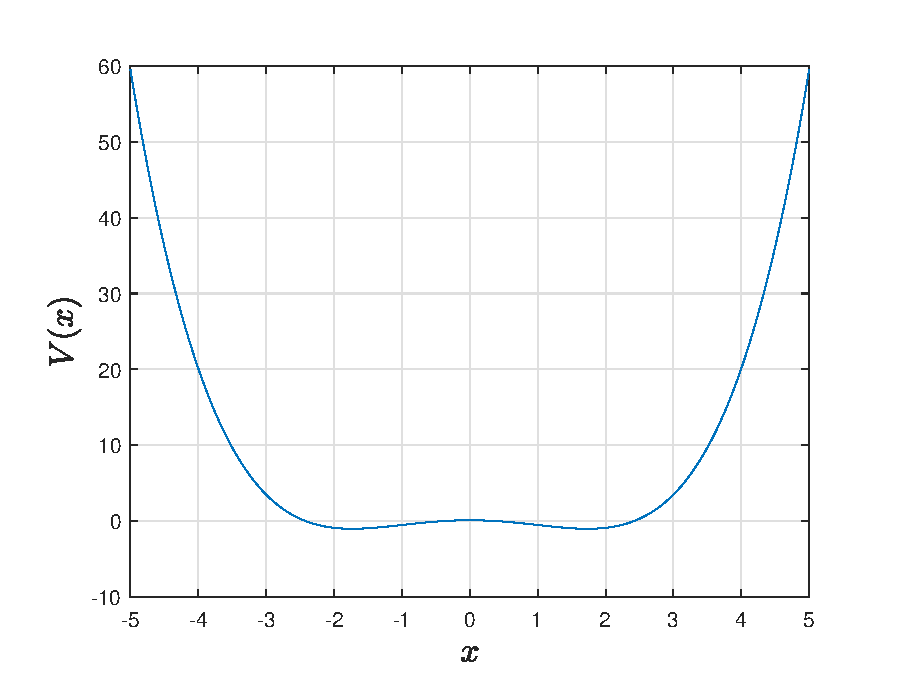
\includegraphics[width=.4\textwidth]{4-Vpot.eps}
        \caption{双势阱的势场.}
        \label{4-Vpot}
    \end{figure}

    \textbf{Numerov方法}:Fortran代码:
    \begin{lstlisting}
program main
    ! solve the Schrodinger equation of a particle in 1-dimension infinite square potential well with Numerov's method

    implicit none
    integer, parameter :: dp = selected_real_kind(8)
    real(dp), parameter :: eps = 1.d-5, dE = 1.d-2

    ! local vars
    real(dp) :: Xmax
    integer :: Nx, i
    real(dp) :: E    ! trial energy
    real(dp) :: dx, ySquareSum
    real(dp), allocatable :: x(:), Vpot(:), y(:), g(:), f(:)
    logical :: yNSignChange = .false., yNSign
    integer :: looptime = 1
    real(dp) :: Eprev1, Eprev2, yprev1, yprev2

    ! executable
    Xmax = -1.d0
    do while (Xmax < 0.d0)
        write(*,*) 'Please indicate the range of x, [-Xmax,Xmax]'
        read(*,*) Xmax
    end do

    Nx = -1
    do while ((Nx <= 0) .or. (mod(Nx, 2) /= 0))
        write(*,*) 'Please specify the # of slices between [0,Xmax], Nx ='
        read(*,*) Nx
    end do

    write(*,*) 'Please give a trial energy E0, the first allowed state with E>E0 will be calculated! E0 ='
    read(*,*) E

    write(*, '(a10,a20,a20)') 'Iteration', 'Energy', 'Boundary value'

    ! memory dynamical allocation
    allocate(x(-Nx:Nx))
    allocate(Vpot(-Nx:Nx))
    allocate(y(-Nx:Nx))
    allocate(g(-Nx:Nx))
    allocate(f(-Nx:Nx))

    dx = Xmax / dble(Nx)
    do i = -Nx, Nx
        x(i) = dx * i
        Vpot(i) = .5d0 * ((x(i)**2 - 1.d0)**2 / 4.d0 - x(i)**2)
    end do

    do while (.true.)
        ! set boundary condition: y(0) and y(1)
        y(-Nx) = 0.d0
        y(-Nx + 1) = 1.d-4

        do i = -Nx, Nx
            g(i) = 2.d0 * (E - Vpot(i))
            f(i) = 1.d0 + g(i) / 12.d0 * dx**2
        end do

        ! Numerov's method
        do i = -Nx + 1, Nx - 1
            y(i + 1) = ((12.d0 - 10.d0 * f(i)) * y(i) - f(i - 1) * y(i - 1)) / f(i + 1)
        end do

        ! renormalize y(x)
        call Simpson(Nx + 1, y(:), dx, ySquareSum)
        y = y / sqrt(ySquareSum)

        ! output to screen
        write(*,'(i10,2f20.8)') looptime, E, y(Nx)

        ! change E
        if (abs(y(Nx)) < eps) then    ! if precision requirement is satisfied
            ! output to file
            open(1, file = '4-wavefunction-Numerov.txt', status = 'unknown')
            do i = -Nx, Nx
                write(1, '(2f20.8)') x(i), y(i)
            end do
            close(1)
            open(2, file = '4-energy-Numerov.txt', status = 'unknown')
            write(2, '(f20.8)') E
            close(2)
            exit
        else
            if (.not. yNSignChange) then    ! if the sign of yN has not changed
                E = E + dE
                if (looptime == 1) then    ! if this is the first loop
                    yNSign = (y(Nx) >= 0)
                    yprev1 = y(Nx)
                else
                    if ((y(Nx) >=0) .neqv. (yNSign)) then    ! if the sign of yN changed this time
                        yNSignChange = .true.
                        E = E - dE
                        Eprev1 = E
                        Eprev2 = E - dE
                        E = E - dE / 2.d0
                    end if
                    yprev2 = yprev1
                    yprev1 = y(Nx)
                end if
            else    ! once the sign of yN has changed
                if (abs(yprev1) <= abs(yprev2)) then
                    Eprev2 = E
                    ! Eprev1 = Eprev1
                    E = (Eprev1 + Eprev2) / 2.d0
                    yprev2 = y(Nx)
                    ! yprev1 = yprev1
                else
                    ! Eprev2 = Eprev2
                    Eprev1 = E
                    E = (Eprev1 + Eprev2) / 2.d0
                    ! yprev2 = yprev2
                    yprev1 = y(Nx)
                end if
            end if
        end if

        looptime = looptime + 1
    end do
end program main

subroutine Simpson(N, y, dx, ySquareSum)
    ! calculate the integral of the square of the wavefunction from -Xmax to Xmax with compound simpson formula

    implicit none
    integer :: N
    real(8), intent(in) :: y(N), dx
    real(8), intent(out) :: ySquareSum

    ! local vars
    integer :: i
    real(8) :: Work(N)

    if (mod(N,2) == 0) then
    ! Simpson does not work for integral of array with even number of elements
        write(*, *) 'Array with even elements, Simpson does not know how to work!'
    end if

    do i = 1,N
        Work(i) = y(i)**2
    end do

    ySquareSum = Work(1) + Work(N)
    do i = 2, N - 1, 2
        ySquareSum = ySquareSum + 4.d0 * Work(i)
    end do
    do i = 3, N - 2, 2
        ySquareSum = ySquareSum + 2.d0 * Work(i)
    end do
    ySquareSum = ySquareSum * dx / 3.d0

end subroutine Simpson
    \end{lstlisting}
    \newpage
    部分计算结果如表.
    \begin{table}[h]
        \centering
        \caption{Numerov方法计算结果:双势阱最低的三个能级}
        \label{4-Numerov}
        \begin{tabular}{cm{.4\textwidth}}
        \hline
        能量 & 波函数图像 \\ \hline
        $-0.32227314$ & 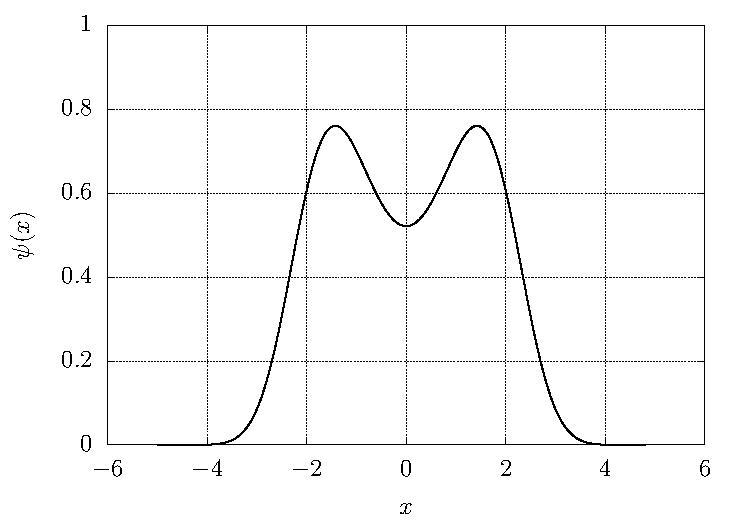
\includegraphics[width=.4\textwidth]{4-Numerov-0.pdf} \\
        $0.83123120$ & 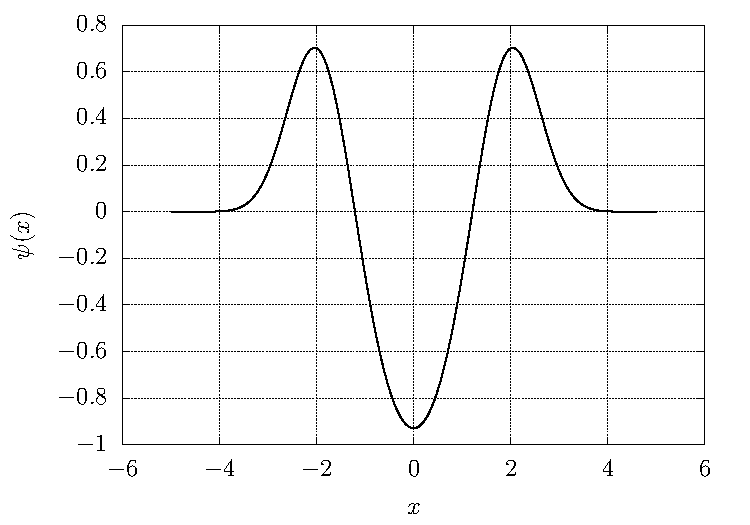
\includegraphics[width=.4\textwidth]{4-Numerov-1.pdf} \\
        $1.71356141$ & 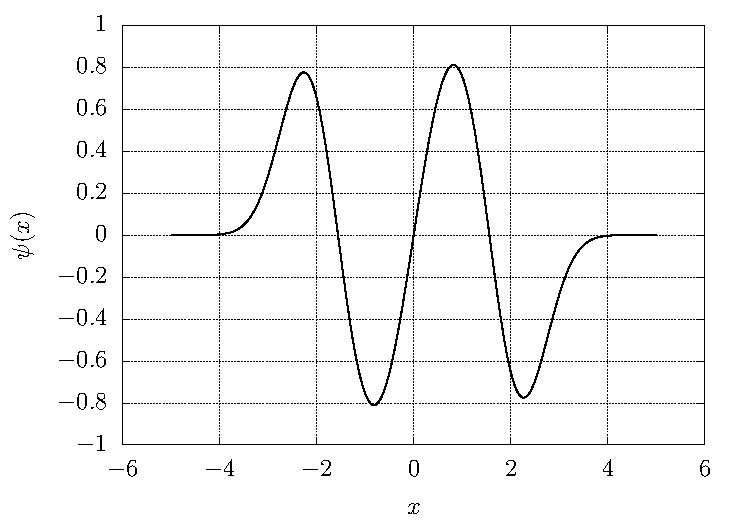
\includegraphics[width=.4\textwidth]{4-Numerov-2.pdf} \\ \hline
        %$2.83622295$ & 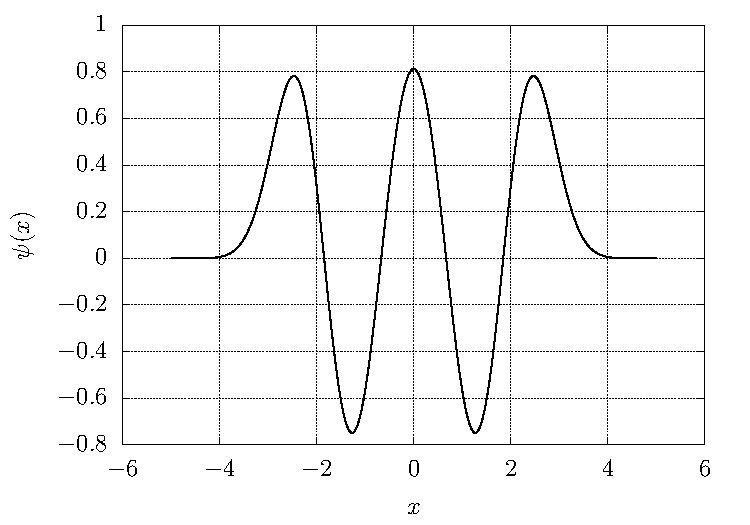
\includegraphics[width=.4\textwidth]{4-Numerov-3.pdf} \\ \hline
        \end{tabular}
        \end{table}

    \textbf{矩阵对角化方法}:以频率为$\omega_0$的量子谐振子的特征波函数
    \begin{equation}
        \label{4-basis}
        \psi_n(x)=H_n\left(\sqrt{\frac{m\omega_0}{\hbar}}x\right)e^{-\frac{m\omega_0}{2\hbar}x^2}
    \end{equation}
    为基矢,其中厄米多项式
    \begin{equation}
        H_n(\xi)=\sum_{m=0}^{[n/2]}\frac{(-1)^mn!}{m!(n-2m)!}(2\xi)^{n-2m}.
    \end{equation}
    我们知道,对于量子谐振子来说,它的特征波函数满足的薛定谔方程为
    \begin{equation}
        -\frac{\hbar^2}{2m}\frac{d^2}{dx^2}\psi_n(x)+\frac{1}{2}m\omega_0^2x^2\psi_n(x)=E_n\psi(x),\quad E=\hbar\omega_0\left(n+\frac{1}{2}\right).
    \end{equation}
    因此将双势阱中粒子的哈密顿在量子谐振子的本征波函数上展开,我们会得到
    \begin{align}
        \label{4-Hamiltonian}
        \nonumber H_{nn'}=&\langle\psi_n^*(x)\rvert H\lvert\psi_{n'}^*(x)\rangle\\
        \nonumber=&\langle\psi_n(x)\rvert\left\{-\frac{\hbar^2}{2m}\frac{d^2}{dx^2}+\frac{m\omega_0^2}{2}\left[\frac{(x^2-x_0^2)^2}{4x_0^2}-x^2\right]\right\}\lvert\psi_{n'}(x)\rangle\\
        \nonumber=&\langle\psi_n(x)\rvert\left\{\left(-\frac{\hbar^2}{2m}\frac{d^2}{dx^2}+\frac{1}{2}m\omega_0^2x^2\right)+\frac{m\omega_0^2}{2}\left[\frac{(x^2-x_0^2)^2}{4x_0^2}-2x^2\right]\right\}\lvert\psi_{n'}(x)\rangle\\
        \nonumber=&\langle\psi_n(x)\rvert\left[\left(-\frac{\hbar^2}{2m}\frac{d^2}{dx^2}+\frac{1}{2}m\omega_0^2x^2\right)\right]\lvert\psi_{n'}(x)\rangle+\langle\psi_n(x)\rvert\frac{m\omega_0^2}{2}\left[\frac{(x^2-x_0^2)^2}{4x_0^2}-2x^2\right]\lvert\psi_{n'}(x)\rangle\\
        \nonumber=&\hbar\omega_0\left(n+\frac{1}{2}\right)\delta_{nn'}+\int_{-\infty}^{+\infty}\psi_n^*(x)\frac{m\omega_0^2}{2}\left[\frac{(x^2-x_0^2)^2}{4x_0^2}-2x^2\right]\psi_{n'}(x)\,dx\\
        \approx&\hbar\omega_0\left(n+\frac{1}{2}\right)\delta_{nn'}+\int_{-Xmax}^{Xmax}\psi_n^*(x)\frac{m\omega_0^2}{2}\left[\frac{(x^2-x_0^2)^2}{4x_0^2}-2x^2\right]\psi_{n'}(x)\,dx
    \end{align}
    综上,我们只在原有矩阵对角化代码的基础上,\sout{按照式\eqref{4-basis}修改基矢组成的矩阵并}按照式\eqref{4-Hamiltonian}修改哈密顿矩阵即可. 但是由于厄米多项式中存在阶乘,当$n$或$m$过大时,会存在溢出的问题,所以先用矩阵对角化方法计算谐振子波函数的近似值来作为基矢,然后再次运用矩阵对角化方法求解双势阱的问题. 代码Fortran:
    \begin{lstlisting}
program main
    ! solve the Schrodinger equation of a particle in an infinite potential well with central barrier with Exact Diagonalization

    implicit none
    integer, parameter :: dp = selected_real_kind(8)
    real(dp), parameter :: pi = acos(-1.d0)

    ! local vars
    integer :: i, j, Nx, LWORK, INFO
    real(dp) :: Xmax, dx, V0
    real(dp), allocatable :: x(:), Vpot(:), Ham(:,:), basis(:,:), W(:), WORK(:)

    integer :: LWORK1, INFO1
    real(dp), allocatable :: x1(:), Vpot1(:), Ham1(:,:), W1(:), WORK1(:)

    ! executable
    Xmax = -1.d0
    do while (Xmax < 0.d0)
        write(*,*) 'Please indicate the range of x, [-Xmax,Xmax]; Xmax ='
        read(*,*) Xmax
    end do

    Nx = -1
    do while (Nx <= 0)
        write(*,*) 'Please specify the # of slices between [0,Xmax], Nx ='
        read(*,*) Nx
    end do

    ! memory dynamical allocation
    allocate(x(-Nx:Nx))
    allocate(Vpot(-Nx:Nx))
    allocate(x1(-Nx - 1:Nx + 1))
    allocate(Vpot1(-Nx - 1:Nx + 1))

    dx = Xmax / dble(Nx)
    do i = -Nx, Nx
        x(i) = dx * dble(i)
        Vpot(i) = .5d0 * ((x(i)**2 - 1.d0)**2 / 4.d0 - x(i)**2)
    end do

    ! calculate the wavefunction of 1D HO
    do i = -Nx - 1, Nx + 1
        x1(i) = dx * dble(i)
        Vpot1(i) = .5d0 * x1(i)**2
    end do

    allocate(Ham1(2 * Nx + 1, 2 * Nx + 1))
    Ham1 = 0.d0
    do i = 1, 2 * Nx + 1
        Ham1(i,i) = Vpot1(i - Nx) + 1.d0 / dx**2
        if (i > i) Ham1(i,i - 1) = -.5d0 / dx**2
        if (i < 2 * Nx + 1) Ham1(i,i + 1) = -.5d0 / dx**2
    end do

    allocate(W1(2 * Nx + 1))
    LWORK1 = 10 * (Nx + 1)
    allocate(WORK1(LWORK1))
    call DSYEV('V','U',2 * Nx + 1, Ham1, 2 * Nx + 1, W1, WORK1, LWORK1, INFO1)

    allocate(basis(2 * Nx + 1, 2 * Nx +1))
    if (INFO1 == 0) then
        do i = 1, 2 * Nx + 1
            do j = 1, 2 * Nx + 1
                basis(i,j) = Ham1(j,i)
            end do
        end do
    else
        write(*, *) 'Diagonalization went wrong! aborting ...'
        stop
    end if

    allocate(Ham(2 * Nx + 1, 2 * Nx + 1))
    Ham = 0.d0
    do i = 1, 2 * Nx + 1
        do j = i, 2 * Nx + 1
            call Simpson(2 * Nx + 1, basis(i, 1:2 * Nx + 1), basis(j, 1:2 * Nx + 1), Vpot(-Nx:Nx) - .5d0, dx, V0)
            Ham(i, j) = V0
            if (i == j) then
                Ham(i, j) = Ham(i, j) + (i - .5d0)
            end if
            Ham(j, i) = Ham(i, j)
        end do
    end do

    allocate(W(2 * Nx + 1))
    LWORK = 10 * Nx
    allocate(WORK(LWORK))
    call DSYEV('V', 'U', 2 * Nx + 1, Ham, 2 * Nx + 1, W, WORK, LWORK, INFO)

    if (INFO == 0) then
        open(unit = 1, file = '4-energy-ExactDiagonalization.txt', status = 'unknown')
        open(unit = 2, file = '4-wavefunction-ExactDiagonalization.txt', status = 'unknown')

        ! multiply the coefficient (which is stored in Ham now) with the basis function to get the wave function
        Ham = matmul(transpose(basis), Ham)

        ! output results
        do i = 1, 2 * Nx + 1
            write(1, '(i4,f20.12)') i, W(i)
            write(2, '(f12.8)', advance = 'no') x(i - Nx -1)
            do j = 1, 2 * Nx + 1
                write(2, '(f12.6)', advance = 'no') Ham(i,j)
            end do
            write(2, *)
        end do
        close(1)
        close(2)
    else
        write(*, *) 'Diagonalization went wrong! aborting ...'
        stop
    end if

    deallocate(Ham)
    deallocate(basis, W, WORK)
    deallocate(x, Vpot)

end program main

subroutine Simpson(N, u, v, Vpot, dx, V0)
    ! calculate the integral of the product of u, v, and Vpot from -Xmax to Xmax with compound simpson formula

    implicit none
    integer :: N
    real(8), intent(in) :: u(N), v(N), Vpot(N), dx
    real(8), intent(out) :: V0

    ! local vars
    integer :: i
    real(8) :: Work(N)

    if (mod(N, 2) == 0) then
    ! Simpson does not work for integral of array with even number of elements
        write(*, *) 'Array with even elements, Simpson does not know how to work!'
    end if

    do i = 1, N
        Work(i) = Vpot(i) * u(i) * v(i)
    end do
     
    V0 = Work(1) + Work(N)
    do i = 2, N - 1, 2
        V0 = V0 + 4.d0 * Work(i)
    end do
    do i = 3, N - 2, 2
        V0 = V0 + 2.d0 * Work(i)
    end do
    V0 = V0 * dx / 3.d0

end subroutine Simpson
    \end{lstlisting}
    部分计算结果如表\ref{4-ExactDiagonalization}.
    \begin{table}[h]
        \centering
        \caption{矩阵对角化方法计算结果:双势阱最低的三个能级}
        \label{4-ExactDiagonalization}
        \begin{tabular}{cm{.4\textwidth}}
        \hline
        能量 & 波函数图像 \\ \hline
        $0.483562389916$ & 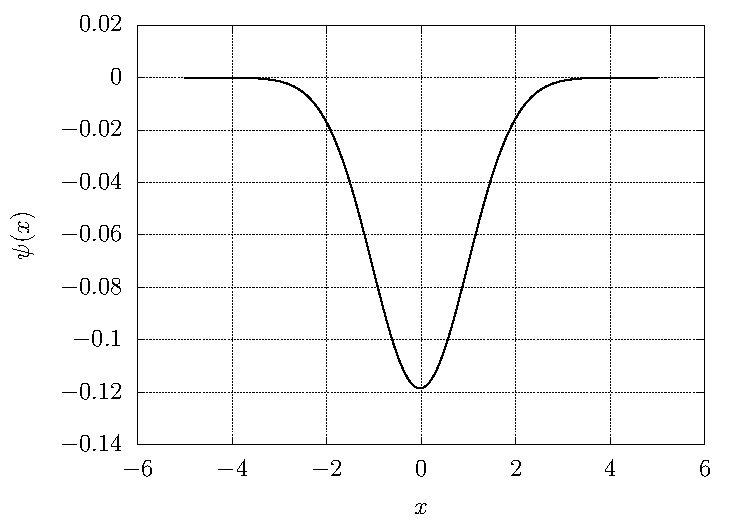
\includegraphics[width=.4\textwidth]{4-ExactDiagonalization-1.pdf} \\
        $1.474199856714$ & 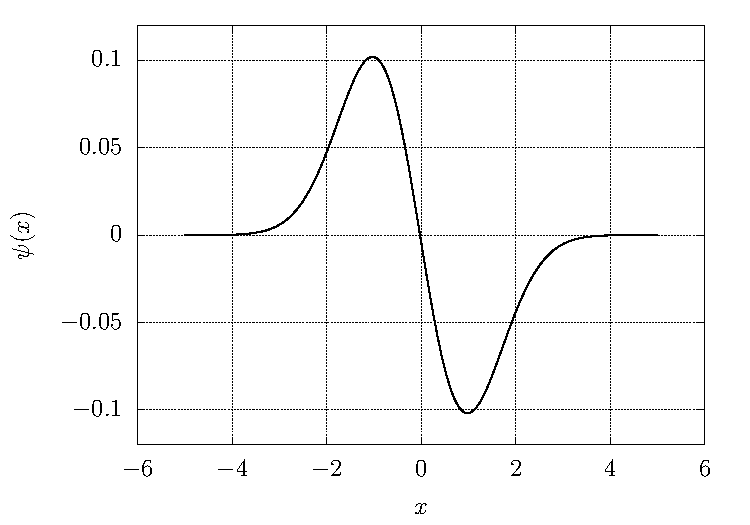
\includegraphics[width=.4\textwidth]{4-ExactDiagonalization-2.pdf} \\
        $2.474189011020$ & 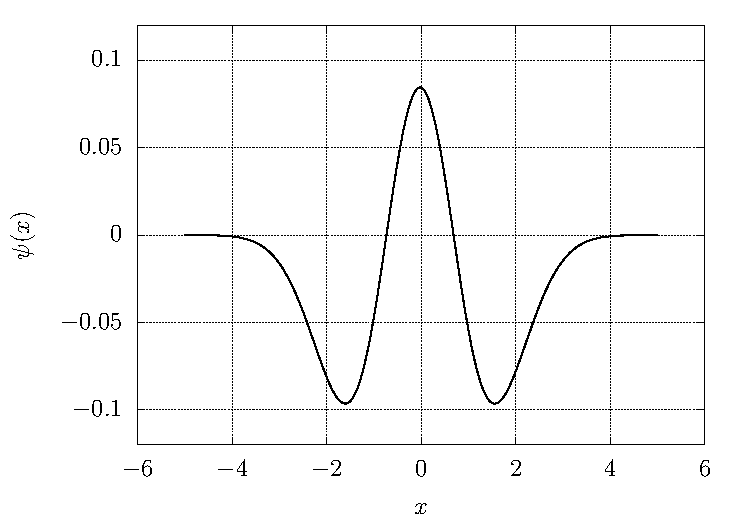
\includegraphics[width=.4\textwidth]{4-ExactDiagonalization-3.pdf} \\ \hline
        \end{tabular}
        \end{table}
        \\双势阱的各能级能量与波函数与量子谐振子的十分相近,即使能量低于中央凸起,粒子依然可以越过中央凸起,体现出量子隧穿的效应.
\end{sol}
\end{document}